\documentclass[11pt]{article}

\usepackage[margin=1in]{geometry}
\usepackage{amsmath,amsthm}
\usepackage{mathtools}
\usepackage{graphicx}
\usepackage{subcaption}
\usepackage{dsfont}
% Old-style journal look, matching the seqtree appendix (OldStandard text+math, small-caps
% headings, run-in paragraph leaders). Requires lualatex -- pinned in .latexmkrc / Makefile.
\usepackage{OldStandard}
\usepackage{unicode-math}
\setmathfont{OldStandard-Math.otf}
\usepackage{titlesec}
\usepackage{tikz}
\usetikzlibrary{positioning, fit}
\usepackage[hidelinks]{hyperref}

\linespread{1.15}
\setlength{\parindent}{2em}
\titleformat{\section}{\normalfont\large\scshape\bfseries}{\thesection.}{0.6em}{}
\titleformat{\subsection}{\normalfont\scshape\bfseries}{\thesubsection.}{0.5em}{}
\titleformat{\paragraph}[runin]{\bfseries\scshape}{}{0pt}{}[.]
\titlespacing*{\paragraph}{\parindent}{0.4em}{0.6em}

\newtheoremstyle{oldplain}{}{}{\itshape}{}{\scshape}{.}{.5em}{}
\newtheoremstyle{oldrem}{}{}{\normalfont}{}{\scshape}{.}{.5em}{}
\theoremstyle{oldplain}
\newtheorem{theorem}{Theorem}
\newtheorem{lemma}{Lemma}
\newtheorem{proposition}{Proposition}
\newtheorem{corollary}{Corollary}
\theoremstyle{oldrem}
\newtheorem{definition}{Definition}
\newtheorem{assumption}{Assumption}
\newtheorem{remark}{Remark}

\DeclareMathOperator{\Poisson}{Poisson}
\DeclareMathOperator{\Binomial}{Binomial}
\DeclareMathOperator{\Var}{Var}
\DeclareMathOperator*{\argmax}{arg\,max}
\DeclareMathOperator{\MI}{I}
\newcommand{\Pzero}{P_{0}}
\newcommand{\Pdata}{P_{\mathrm{data}}}
\newcommand{\R}{\mathbb{R}}
\newcommand{\E}{\mathbb{E}}
\newcommand{\Prob}{\mathbb{P}}
\newcommand{\one}{\mathds{1}}
\newcommand{\dTCR}{d_{\mathrm{TCR}}}
\newcommand{\ESS}{\mathrm{ESS}}

\title{\scshape Presentation-aware E-values, cross-allele pseudosequence diffusion, and
proteome-scale peptide matching for peptide--MHC analysis}
\author{Mikhail Shugay\textsuperscript{1,2,3}\thanks{Correspondence:
  \href{mailto:mikhail.shugay@gmail.com}{mikhail.shugay@gmail.com}}}
\date{%
  \small
  \textsuperscript{1}Institute of Translational Medicine, Russian National Medical State University, Moscow, Russia\\
  \textsuperscript{2}Department of Genomics of Adaptive Immunity, Shemyakin--Ovchinnikov Institute of Bioorganic Chemistry RAS, Moscow, Russia\\
  \textsuperscript{3}Institute of Molecular Biology NAS RA, Erevan, Armenia\\[6pt]
  \normalsize\textit{mhcmatch technical appendix}%
}

\begin{document}
\maketitle

\begin{abstract}
This appendix develops the mathematical and statistical theory of \texttt{mhcmatch}, the applied
peptide--MHC layer built on the \texttt{seqtree} fuzzy-search substrate. We take as given the
control-calibrated E-value of the \texttt{seqtree} appendix (\texttt{evalue.tex}) and specialize it
to MHC \emph{presentation}, whose null is allele-conditional and anchor-constrained. We restate the
anchor / TCR-facing decomposition and the per-allele presentation-aware E-value (the \emph{forward}
restriction problem), then the \emph{reverse} problem---peptide to presenting allele---as a
neighbour-vote posterior with a binomial-tail confidence E-value, together with its non-binder
filter and class-II promiscuity treatment. The central contribution is a \emph{cross-allele
diffusion} model: each allele is represented by its 34-residue groove pseudosequence, and per-anchor
preference distributions are smoothed by kernel-weighted empirical-Bayes shrinkage toward
groove-similar alleles, with the per-anchor relevance of each groove position \emph{learned} from
data (a mutual-information feature importance that separates, e.g., the MHC-I B-pocket governing P2
from the F-pocket governing P$\Omega$). This rescues rare alleles with few peptides---lifting the
\texttt{seqtree} limitation that distinct alleles are distinct, never-pooled nulls---and we give its
hierarchical-Bayes interpretation, effective sample size, limiting cases, and bias--variance
trade-off. We then treat proteome-scale scanning (sliding-window presentation with multiple-testing
control; near-exact neoantigen source identification), motif logos with length distributions, the
composition rules for the planned stability / affinity / cleavage / expression / immunogenicity
predictors, and the benchmark protocol against NetMHCpan, NetMHCIIpan, MixMHCpred and MixMHC2pred.
\end{abstract}

\section{Scope and relation to the substrate}\label{sec:scope}
\texttt{seqtree} provides a payload-agnostic fuzzy-search core and a control-calibrated E-value: for
a query $q$ and a scope $\theta$, with an empirical background $\Pzero$ estimated from a matched
control of size $M$ and a target set of size $N$, the expected number of chance neighbours is
$\widehat E(q,\theta)=(N/M)\,n_C(q,\theta)$, with $p_{\mathrm{any}}=1-e^{-\widehat E}$ and
$p_{\mathrm{enrich}}=\Prob(\Poisson(\widehat E)\ge n_D)$ (\texttt{seqtree} appendix, Def.\ of the
E-value; Poisson/Chen--Stein bound; Karlin--Altschul~\cite{Karlin1990,Altschul1990} as the
i.i.d.\ special case). We do not re-derive that theory; we \emph{specialize} it.

For peptide--MHC the relevant background is not V(D)J generation but \emph{presentation}, which is
allele-conditional and constrains the anchor positions. \texttt{mhcmatch} owns four developments on
top of the substrate: (i) the productionized forward/reverse presentation E-value
(\S\ref{sec:forward}--\ref{sec:reverse}); (ii) the cross-allele \emph{pseudosequence diffusion}
model that pools statistics across groove-similar alleles (\S\ref{sec:diffusion}, the headline);
(iii) proteome-scale scanning and near-exact source identification (\S\ref{sec:proteome}); and
(iv) motif logos (\S\ref{sec:logos}). Planned predictors and the comparison protocol are
\S\ref{sec:predictors}--\ref{sec:bench}; limitations are \S\ref{sec:limits}.

\section{Anchor decomposition and the per-allele presentation E-value}\label{sec:forward}
A presented peptide of length $L$ factorizes $\sigma=(\sigma_A,\sigma_T)$ into MHC-facing
\emph{anchors} $A(a,L)$ and TCR-facing positions $T$. For class~I the buried anchors are
$\{\mathrm{P2},\mathrm{P}\Omega\}$ (the B- and F-pockets); for the class~II 9-mer core they are
$\{\mathrm{P1},\mathrm{P4},\mathrm{P6},\mathrm{P9}\}$. \emph{Presentation} fixes $\sigma_A$;
\emph{recognition} reads $\sigma_T$. Dolton~et~al.~\cite{Dolton2023} exhibit one HLA-A\*02:01 TCR
cross-reacting with three epitopes through a shared central motif with the anchors irrelevant, which
motivates two complementary maskings, each realized by a per-position weight vector $w$ over a
\texttt{seqtree} \texttt{PositionalMatrix}:
\begin{equation}\label{eq:masks}
  \text{(recognition)}\quad w_i=\one[i\in T];\qquad
  \text{(presentation)}\quad w_i=\one[i\in A(a,L)].
\end{equation}
In \texttt{mhcmatch} these are exposed by \texttt{Store.decompose}, which returns both readouts with
the masked positions written as the spare symbol \texttt{X}.

\paragraph{Forward problem.} For a candidate restriction allele $a$ with an anchor-masked presented
control $C_a$ of size $M_a$ and target peptidome of size $N_a$, the presentation-aware E-value is the
substrate E-value on allele-restricted, anchor-conditioned indices,
\begin{equation}\label{eq:forward}
  \widehat E(q,\theta;a)=\frac{N_a}{M_a}\,n_{C_a}(\sigma_T,\theta),\qquad
  p_{\mathrm{enrich}}=\Prob\!\big(\Poisson(\widehat E)\ge n^T_{D_a}\big),
\end{equation}
i.e.\ significance is computed on the TCR-facing readout only, so shared anchors (presentation, not
recognition) do not inflate within-allele hits. The analytic null for rare $a$ is taken up in
\S\ref{sec:diffusion}.

\section{Reverse problem: peptide to presenting allele}\label{sec:reverse}
The forward E-value answers ``is $q$ a binder of a \emph{given} $a$?''. Restriction prediction asks
the reverse: which alleles present $q$? We flip the weights in~\eqref{eq:masks} to the
\emph{presentation} mode and index reference peptides by their anchor signature
(\texttt{layout.presentation\_features}; class~I N/C-pocket residues
$\mathrm{P1\,P2\,P3}$, $\mathrm{P}(\Omega{-}1)$, $\mathrm{P}\Omega$, class~II core
$\mathrm{P1\,P4\,P6\,P9}$). For a query
we widen the scope on its signature until it has $n\in[10,100]$ non-exact neighbours, and tally their
alleles, $k_a$ votes out of $n$.

\begin{definition}[Ranking and confidence]\label{def:reverse}
The \emph{ranking} score is the neighbour vote fraction $\hat p(a\mid q)=k_a/n$, a posterior over the
panel. The \emph{confidence} score is the per-allele enrichment over the panel background frequency
$f_a$,
\begin{equation}\label{eq:conf}
  E_a=-\log_{10}\Prob\!\big(\Binomial(n,f_a)\ge k_a\big),
\end{equation}
the upper binomial tail; a peptide binds $a$ iff $E_a\ge-\log_{10}\alpha$ and $k_a>0$.
\end{definition}

\begin{remark}[Why vote fraction, not enrichment, ranks]
On a skewed panel the dominant true allele has a large expected count $n f_a$, so the
enrichment~\eqref{eq:conf} \emph{penalises} it; the vote fraction does not. Hence $\hat p$ ranks and
$E_a$ gates. This separation, validated on \texttt{pmhc\_data} (per-(peptide, allele) ROC-AUC
$0.90$--$0.99$, \texttt{seqtree/bench/bench\_mhc\_guess.py}), is what \texttt{Store.restriction}
implements.
\end{remark}

\paragraph{Class-II register trick.} The class-II core register inside a longer peptide is unknown;
full deconvolution clusters it~\cite{Andreatta2017,Alvarez2019}. We use a one-pass proxy: pick the
single 9-mer window whose P1 is a large hydrophobic and whose P4/P6/P9 avoid Pro/Gly, and take that
core's $\{$P1,P4,P6,P9$\}$. Committing to one register makes an allele's peptides share a consistent
signature and is what lifts class-II ROC-AUC into the $0.9$ range.

\paragraph{Non-binder filter and promiscuity.} A peptide that binds \emph{no} panel allele has small
$\max_a E_a$ (real-vs-random rejection); one that does not bind a \emph{specific} $a$ has
$E_a<-\log_{10}\alpha$. The global statistic $E_{\mathrm{glob}}=\sum_a 10^{-E_a}$ is the expected
number of panel alleles presenting $q$ by chance. Class~II is genuinely multi-label (an open groove
with loosely specified pockets presents one peptide on many alleles), so the panel positive set is
\emph{every} observed restricting allele and the non-binder test is ``binds none of the panel''.

\subsection{Where the E-value is used: significance vs ranking}\label{sec:evalue-role}
The E-value is a calibrated \emph{significance}---an expected chance count and its Poisson tail
(\S\ref{sec:forward})---not a discriminative score, and the two answer different questions.
\emph{Ranking} (the diffused anchor log-odds, or the neighbour vote) \emph{orders} candidates and is
the better discriminator: for allele prediction the log-odds ranks best (\S\ref{sec:bench}), and for
telling binders from random non-binders the max-over-panel presentation score reaches AUROC
$\approx0.80$ (real held-out peptides vs $10^4$ corpus-frequency random peptides). The \emph{E-value}
answers ``is this many hits more than chance against the right background?''---it is what one
\emph{reports} when significance and multiplicity matter:
\begin{itemize}
  \item \textbf{Molecular mimicry and self/proteome search} (\S\ref{sec:proteome}): for a neoantigen,
  \texttt{find\_mimics} reports the expected number of TCR-facing homologs in a self or pathogen set
  against the \emph{per-allele presented} background, with $p_{\mathrm{enrich}}$ and the rule of three
  for empty controls. Rank cannot say whether a shared motif is surprising; the E-value deflates
  motifs common in the allele's peptidome, elevates surprisingly shared ones, and lets one scan whole
  proteomes under FWER/FDR control. This is the principal reason to carry an E-value.
  \item \textbf{Binder vs non-binder} uses \emph{both}: the diffused log-odds (or its max over the
  panel) to \emph{rank / discriminate}, and the per-allele enrichment $E_a$---or the global
  $E_{\mathrm{glob}}$ for ``binds nothing''---to \emph{gate} with a calibrated threshold and control
  error across a panel or proteome. Empirically the score is the better \emph{discriminator}
  (enrichment-vs-background penalizes data-rich alleles and needs neighbours), while the E-value
  supplies the defensible cut-off and the multiple-testing control the bare score lacks. They
  compose: rank by score, then threshold by $E$ / FDR.
\end{itemize}

\section{MHC pseudosequence model and cross-allele diffusion}\label{sec:diffusion}
\texttt{seqtree} deliberately treats distinct alleles as distinct, never-pooled nulls. This is
correct but wasteful: rare alleles carry few presented peptides, so both~\eqref{eq:forward}
and~\eqref{eq:conf} are noisy exactly where data are thin---the equity problem of
Glynn~et~al.~\cite{Glynn2025}. \texttt{mhcmatch} lifts the limitation by making the allele a
\emph{sequence} the same engine can compare, and diffusing statistics along groove similarity.

\paragraph{Pseudosequence.} Each allele $a$ is represented by its NetMHCpan-style 34-residue groove
pseudosequence $s_a\in\Sigma^{34}$~\cite{Reynisson2020}: the polymorphic, peptide-contacting
positions (class~I $\alpha_1/\alpha_2$; class~II $\alpha_1$ + $\beta_1$). Per-allele binding can be
predicted from $s_a$ alone~\cite{Glynn2025,BassaniSternberg2017}, so groove distance is a meaningful
allele distance.

\subsection{Anchor-factored similarity kernel}
The presentation motif factorizes by pocket: anchor $j$'s residue preference is governed by the
groove positions lining pocket $j$, and different pockets are spatially separated (the class-I
B-pocket sets P2, the F-pocket sets P$\Omega$). We therefore use a \emph{per-anchor} kernel rather
than one global allele distance. For anchor $j$ let $w_j\in\R_{\ge0}^{34}$ weight the groove
positions, and define
\begin{equation}\label{eq:kernel}
  d_j(a,b)=\sum_{p=1}^{34} w_{j,p}\,\delta(s_{a,p}, s_{b,p}),\qquad
  K_j(a,b)=\exp\!\big(-d_j(a,b)/h_j\big),
\end{equation}
where $\delta(x,y)=s(x,x)+s(y,y)-2 s(x,y)$ is the BLOSUM62 Gram distance (zero on identity, small for
conservative substitutions, large for dissimilar residues; normalized so an average substitution
costs $\approx 1$), evaluated through \texttt{seqtree}'s substitution matrix
(\texttt{SubstitutionMatrix.penalty}, exposed for this use). Bandwidth $h_j>0$; ambiguous positions
$\texttt{X}$ are skipped. Replacing $\delta$ with the identity indicator $\one[x\neq y]$ gives the
plain Hamming variant, and $w_j\equiv 1$ a single un-factored kernel.

\begin{definition}[Learned per-anchor relevance]\label{def:weights}
Let $A_j$ be the allele's modal residue at peptide anchor $j$ (from its presented set) and $S_p$ the
groove residue at pseudosequence position $p$, both viewed as categorical variables over the allele
panel. The relevance of position $p$ to anchor $j$ is the mutual information
\begin{equation}\label{eq:mi}
  w_{j,p}\;\propto\;\MI(S_p;A_j)=\sum_{x,y}\hat{\Prob}(S_p{=}x,A_j{=}y)\,
  \log_2\frac{\hat{\Prob}(S_p{=}x,A_j{=}y)}{\hat{\Prob}(S_p{=}x)\,\hat{\Prob}(A_j{=}y)},
\end{equation}
normalized to mean one over $p$. Equivalently $w_j$ may be fit by maximizing the held-out predictive
log-likelihood of the shrinkage model below under an $\ell_1$/entropy penalty, which selects each
anchor's pocket positions. \eqref{eq:mi} is the ``feature importance'' that says which groove
residues drive P2 versus P$\Omega$.
\end{definition}

\subsection{Kernel-shrinkage pooling}
Write $\theta_{a,j}$ for allele $a$'s empirical residue distribution at anchor $j$ over its $n_a$
peptides. We shrink it toward groove-similar alleles:
\begin{equation}\label{eq:shrink}
  \hat\theta_{a,j}
  =\frac{n_a\,\theta_{a,j}+\sum_{b\neq a}K_j(a,b)\,n_b\,\theta_{b,j}}
        {n_a+\sum_{b\neq a}K_j(a,b)\,n_b},
  \qquad
  \ESS_{a,j}=n_a+\sum_{b\neq a}K_j(a,b)\,n_b .
\end{equation}
\begin{proposition}[Hierarchical-Bayes reading and limits]\label{prop:shrink}
\eqref{eq:shrink} is the posterior mean of a Dirichlet--multinomial in which the neighbour-weighted
counts form the prior pseudocounts: $\hat\theta_{a,j}=\E[\theta\mid \text{counts}]$ with
concentration $\ESS_{a,j}$. As $h_j\to0$, $K_j(a,b)\to0$ for $b\neq a$ and
$\hat\theta_{a,j}\to\theta_{a,j}$ (no pooling); as $h_j\to\infty$, $K_j(a,b)\to1$ and
$\hat\theta_{a,j}\to(\sum_b n_b\theta_{b,j})/\sum_b n_b$ (the global pool).
\end{proposition}
\noindent (Both limits are implemented and unit-tested in \texttt{Pseudoseq.shrink}.)

\begin{proposition}[Bias--variance and bandwidth]\label{prop:bv}
Treat each $\theta_{b,j}$ as an unbiased estimate of allele $b$'s truth $\theta^\star_{b,j}$ with
variance $\propto 1/n_b$. The pooled estimator has variance $O(1/\ESS_{a,j})$ and bias
$\big\|\sum_b \kappa_b(\theta^\star_{b,j}-\theta^\star_{a,j})\big\|$, where
$\kappa_b=K_j(a,b)n_b/\ESS_{a,j}$ is the borrowed mass. The mean-squared error is minimized by
borrowing more (smaller effective $h_j$ penalty) when $n_a$ is small and groove neighbours are close,
and less when $n_a$ is large; calibrating $h_j$ by cross-validated predictive likelihood realizes
this trade-off automatically.
\end{proposition}

\paragraph{Bounded-concentration variant (the practical default).} The counts-weighted
form~\eqref{eq:shrink} lets one deep neighbour ($K_j n_b\gg n_a$) overwrite a rare allele's own
peptides. We therefore default to a fixed prior strength $\tau$: shrink toward the kernel-weighted
neighbour mean $m_{a,j}=\big(\sum_{b}K_j(a,b)n_b\theta_{b,j}\big)/\sum_b K_j(a,b)n_b$,
\begin{equation}\label{eq:shrink-tau}
  \hat\theta_{a,j}=\frac{n_a\,\theta_{a,j}+\tau\,m_{a,j}}{n_a+\tau},
\end{equation}
so borrowing adds at most $\tau$ pseudocounts and vanishes automatically as $n_a$ grows
(Prop.~\ref{prop:bv}). Empirically (\texttt{bench/bench\_diffusion.py}; human, allele-split
held-out rank AUC with the BLOSUM-scored, MI-weighted kernel~\eqref{eq:kernel}, $\tau=10$, $h=2$, the
per-allele score being the anchor log-odds over the N/C pocket footprint
$\{$P1,P2,P3,P$(\Omega{-}1)$,P$\Omega\}$) the diffusion lifts the AUC of \emph{rare} MHC-I alleles
($\le 30$ peptides) from $0.94$ to $0.96$ on the high-confidence ($\ge2$-publication) set while
leaving \emph{medium} ($31$--$199$) and \emph{frequent} alleles unchanged ($\approx0.97$); the gain
decays smoothly as an allele's own data grows and frequent alleles are never harmed. The class~II
AUC gains are smaller throughout ($\le0.02$, rare $0.77\!\to\!0.77$), consistent with the harder
class~II problem (Fig.~\ref{fig:diffauc}). Exclusion
is \emph{per-pMHC and benchmark-only}: only the held-out (epitope, allele) pair is dropped from
training---the same epitope presented by another allele is a distinct, legitimate pMHC and is kept,
so the diffusion may borrow that co-presentation (the real cross-allele transfer we measure); the
production model trains and votes on all data. The richer pocket footprint matters: with the two
primary anchors alone ($\{$P2,P$\Omega\}$) the full-set rare gain nearly vanishes, whereas the
auxiliary pocket-proximal positions make per-allele estimation sparser---so diffusion has more to
rescue. The data-rescue is safe: it never lowers a well-sampled allele's AUC.

\paragraph{Allele prediction (top-$k$, promiscuity-aware, cross-validated).} Cast as the reverse
problem---for each held-out pMHC $(p,a)$ rank all panel alleles for $p$ and ask whether the held-out
allele $a$ is recovered in the top-$k$. We use \emph{5-fold} cross-validation, pooling each pMHC's
single out-of-fold prediction, capped per allele so rare alleles are represented and frequent ones
do not dominate (\texttt{bench/tune\_diffusion.py}; per-panel tables in \texttt{bench/results/}).
Because peptides are promiscuous we score \emph{recovery@5} split by allele rarity. For MHC-I the
diffusion lifts \emph{rare}-allele recovery@5 from $0.47$ to $0.75$ (shortlist) and $0.30$ to $0.44$
(full tier), at a small frequent cost ($\approx-0.02$) and roughly flat overall top-5
($\approx0.85$/$0.64$). The \emph{ranker} is the diffused anchor log-odds itself, not the neighbour
vote: on a novel peptide the vote tally has few same-allele signature neighbours, so vote-first
ranking buries the true allele (top-5 $0.87$, rare recovery@5 $0.25$ on a single split) whereas the
diffused log-odds scores every allele directly. A grid sweep selects $h=2,\tau=10$, BLOSUM
(marginally over identity), as optimal. Class~II remains hard (recovery@5 $\approx0.47$, diffusion
near-neutral, top-5 $\approx0.25$) and mouse is too few-allele to be conclusive (high CV variance):
both are targets for the structure-based extension. Top-1 is \emph{not} the right yardstick here
(promiscuity makes several alleles correct); top-5/recovery@5 is.

\paragraph{Per-locus calibration.} A single global $(h,\tau)$ need not be optimal for every locus.
A per-locus grid (\texttt{tune\_diffusion.py --by-locus}) shows the loci do differ---HLA-B tolerates
wider borrowing ($h{=}2$) than HLA-A/C ($h{=}0.5$), and most prefer a weaker prior ($\tau{=}5$)---but
the per-locus rare sets on a single split are small and the estimates noisy (HLA-A's apparent
recovery@5 of $1.0$ is a tiny-sample artifact). We therefore keep the cross-validated global
$h{=}2,\tau{=}10$ as the production default and treat validated per-locus tuning (a CV grid per locus,
needing more data) as a calibration refinement rather than promoting single-split optima.

\paragraph{Zero-shot transfer (leave-one-allele-out).} The sharpest test of the rescue removes
\emph{every} peptide of a target allele from training and scores its held-out peptides from groove
neighbours alone (\texttt{bench/transfer.py}). On $30$ human MHC-I alleles the diffused model reaches
real-vs-random AUROC $0.95$ with \emph{no} data for the target allele (the data-free raw model is
uninformative, $0.22$), and transfer stays strong even when the nearest trained groove neighbour is
only moderately similar ($0.94$ at kernel $<0.5$ vs $0.96$ at $\ge0.5$): a genuinely novel allele is
predicted purely from its pseudosequence---the limiting case of the rare-allele rescue.

\begin{figure}[ht]\centering
  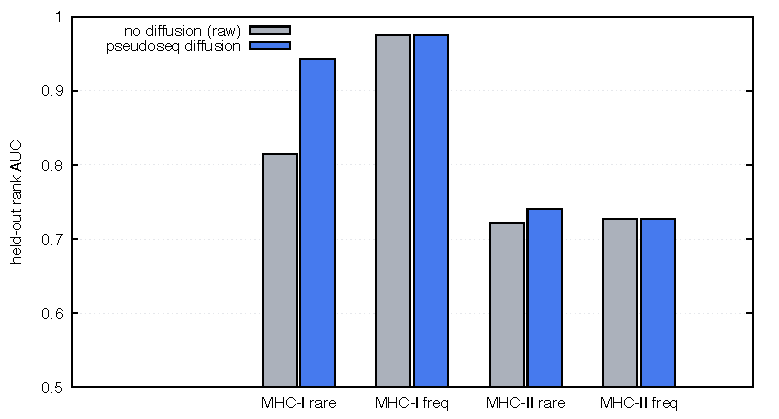
\includegraphics[width=0.8\linewidth]{diffusion_auc.pdf}
  \caption{Held-out rank AUC for rare ($\le30$ peptides), medium ($31$--$199$) and frequent
  ($\ge200$) alleles, without (raw, grey) and with (blue) pseudosequence diffusion, allele-split.
  MHC-I on the $\ge2$-publication set, MHC-II on the full set. Diffusion lifts rare alleles and leaves
  medium and frequent alleles essentially unchanged in both classes---the gain decays smoothly as an
  allele's own data grows. \texttt{bench/bench\_diffusion.py}.}
  \label{fig:diffauc}
\end{figure}

\paragraph{Bayesian reading (in plain terms).} The shrinkage~\eqref{eq:shrink-tau} is exactly a
Bayesian posterior mean. Treat each allele's anchor-$j$ preference $\theta_{a,j}$---the probabilities
of each amino acid in pocket $j$---as \emph{unknown}. Before seeing allele $a$'s own peptides we
expect it to resemble its groove neighbours, so we put a prior centred on the kernel-weighted
neighbour mean $m_{a,j}$ with strength $\tau$ (measured in pseudo-peptides); the allele's $n_a$
observed peptides then update that belief. With the conjugate Dirichlet--multinomial model
\begin{equation}\label{eq:bayes}
  \theta_{a,j}\sim\mathrm{Dirichlet}(\tau\,m_{a,j}),\quad
  \sigma_{i,j}\mid\theta_{a,j}\sim\mathrm{Categorical}(\theta_{a,j}),\quad
  \theta_{a,j}\mid\{\sigma_{i,j}\}\sim\mathrm{Dirichlet}(\tau\,m_{a,j}+c_{a,j}),
\end{equation}
where $c_{a,j}(r)$ counts peptides of $a$ with residue $r$ at pocket $j$ ($\sum_r c_{a,j}(r)=n_a$),
the posterior mean is \emph{precisely}~\eqref{eq:shrink-tau}. A data-rich allele ($n_a\gg\tau$)
ignores the prior and keeps its own motif; a data-poor one ($n_a\ll\tau$) leans on its neighbours.
The bandwidth $h$ (how far similarity reaches) and the strength $\tau$ (how much to borrow) are the
only knobs (Fig.~\ref{fig:bayes}).

\begin{figure}[ht]\centering
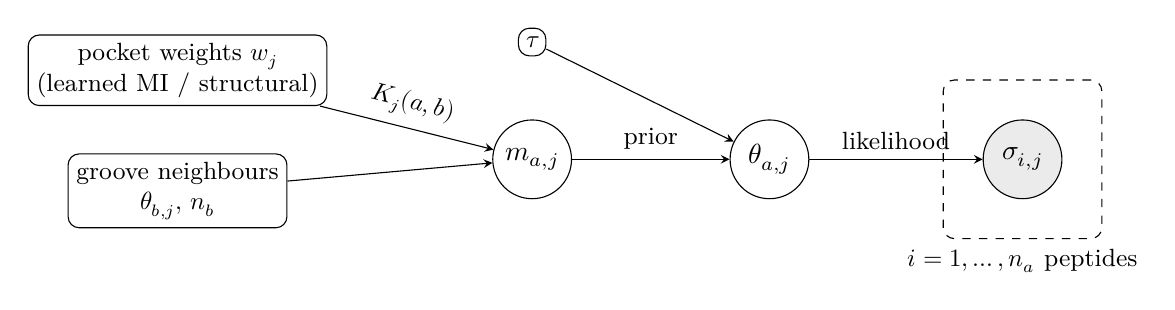
\begin{tikzpicture}[>=stealth,
    latent/.style={draw, circle, minimum size=10mm, inner sep=1pt},
    obs/.style={latent, fill=black!8},
    hyp/.style={draw, rounded corners, align=center, font=\small, inner sep=3pt}]
  \node[hyp] (nb) {groove neighbours\\$\theta_{b,j},\,n_b$};
  \node[hyp, above=6mm of nb] (w) {pocket weights $w_j$\\(learned MI / structural)};
  \node[latent, right=26mm of nb, yshift=4mm] (m) {$m_{a,j}$};
  \node[hyp, above=8mm of m] (tau) {$\tau$};
  \node[latent, right=20mm of m] (th) {$\theta_{a,j}$};
  \node[obs, right=22mm of th] (s) {$\sigma_{i,j}$};
  \node[draw, dashed, rounded corners, fit=(s), inner sep=5mm,
        label={[font=\small]below:$i=1,\dots,n_a$ peptides}] (pl) {};
  \draw[->] (w) -- node[above, font=\small, sloped] {$K_j(a,b)$} (m);
  \draw[->] (nb) -- (m);
  \draw[->] (m) -- node[above, font=\small] {prior} (th);
  \draw[->] (tau) -- (th);
  \draw[->] (th) -- node[above, font=\small] {likelihood} (s);
\end{tikzpicture}
\caption{Graphical model behind the diffusion shrinkage, fit independently per pocket $j$. The
per-pocket groove weights $w_j$---learned by mutual information~\eqref{eq:mi} or measured from
structures (\S\ref{sec:pockets})---set the BLOSUM-scored similarity kernel $K_j(a,b)$~\eqref{eq:kernel};
the kernel-weighted neighbour mean $m_{a,j}$ and the strength $\tau$ form a Dirichlet \emph{prior} on
the allele's pocket-$j$ residue distribution $\theta_{a,j}$; the $n_a$ observed anchor residues
$\sigma_{i,j}$ (shaded) are the \emph{likelihood}. The posterior mean is the shrinkage
estimator~\eqref{eq:shrink-tau}: rare alleles borrow from groove-similar neighbours, well-sampled
alleles do not.}
\label{fig:bayes}
\end{figure}

\paragraph{Pooled null and restored E-value.} For a rare allele the analytic presented null is built
from the shrunk anchor marginals: assuming approximate position independence in the anchor block
(the maximum-entropy presented distribution of~\cite{TiffeauMayer2026} conditioned on the motif),
$\widehat{\Pzero}(\sigma_A\mid a)\approx\prod_{j}\hat\theta_{a,j}(\sigma_{A_j})$, which feeds a usable
$\widehat E$ in~\eqref{eq:forward}--\eqref{eq:conf} where the raw per-allele control was too small.
The estimator is a smoothed null: its bias is controlled by the borrowed mass on dissimilar alleles
(Prop.~\ref{prop:bv}), vanishing as the panel around $a$ becomes dense and groove-tight. In the
production reverse problem (\texttt{Store.restriction}, \texttt{diffuse=True}) the shrunk anchor
log-odds both \emph{ranks} the alleles and, with the neighbour enrichment~(Def.~\ref{def:reverse}),
\emph{gates} binders (binder iff vote-significant or anchor log-odds $>0$). On held-out (novel)
peptides the anchor log-odds is the better ranker: the vote tally needs same-allele signature
neighbours, which are sparse for a genuinely new peptide, so vote-first ranking buries the true
allele (top-5 $0.87$, rare recovery@5 $0.25$), whereas ranking by the diffused log-odds scores every
allele directly (top-5 $0.95$, rare recovery@5 $0.88$; \S\ref{sec:bench}). Vote thus serves the
\emph{confidence gate}, not the ranking.

\subsection{Clustering and promiscuity}
Thresholding $K_j$ (or the un-factored $K$) yields single-linkage allele \emph{clusters} of
functionally similar alleles (\texttt{Pseudoseq.cluster}). A peptide presented across a cluster is
\emph{promiscuous}; its promiscuity is the spread of its positive alleles over the clustering, and
the cluster is the natural unit over which to pool nulls when per-allele data are thin (especially
class~II). This is the principled cross-allele similarity that the substrate omits.
Fig.~\ref{fig:promiscuity} renders this as an allele network---edges are the MI-weighted,
BLOSUM-scored kernel~\eqref{eq:kernel} above a soft/hard threshold, communities are greedy-modularity
clusters~\cite{Clauset2004}---which recover the classical HLA supertypes (A2, A3, B7, B27, B44, \dots), the
structural basis of cross-allele promiscuity. Mouse panels are few and groove-divergent, so they
form no such communities. The kernel communities are well separated (partition modularity $Q=0.94$
human MHC-I, $0.90$ class~II) and respect allele structure---about half of same-two-field-family
allele pairs co-cluster, the remainder splitting only because distant family members fall below the
edge threshold (\texttt{bench/promiscuity\_graph.py}); a quantitative map to a curated supertype set
is the natural external-data validation.

\begin{figure}[ht]\centering
  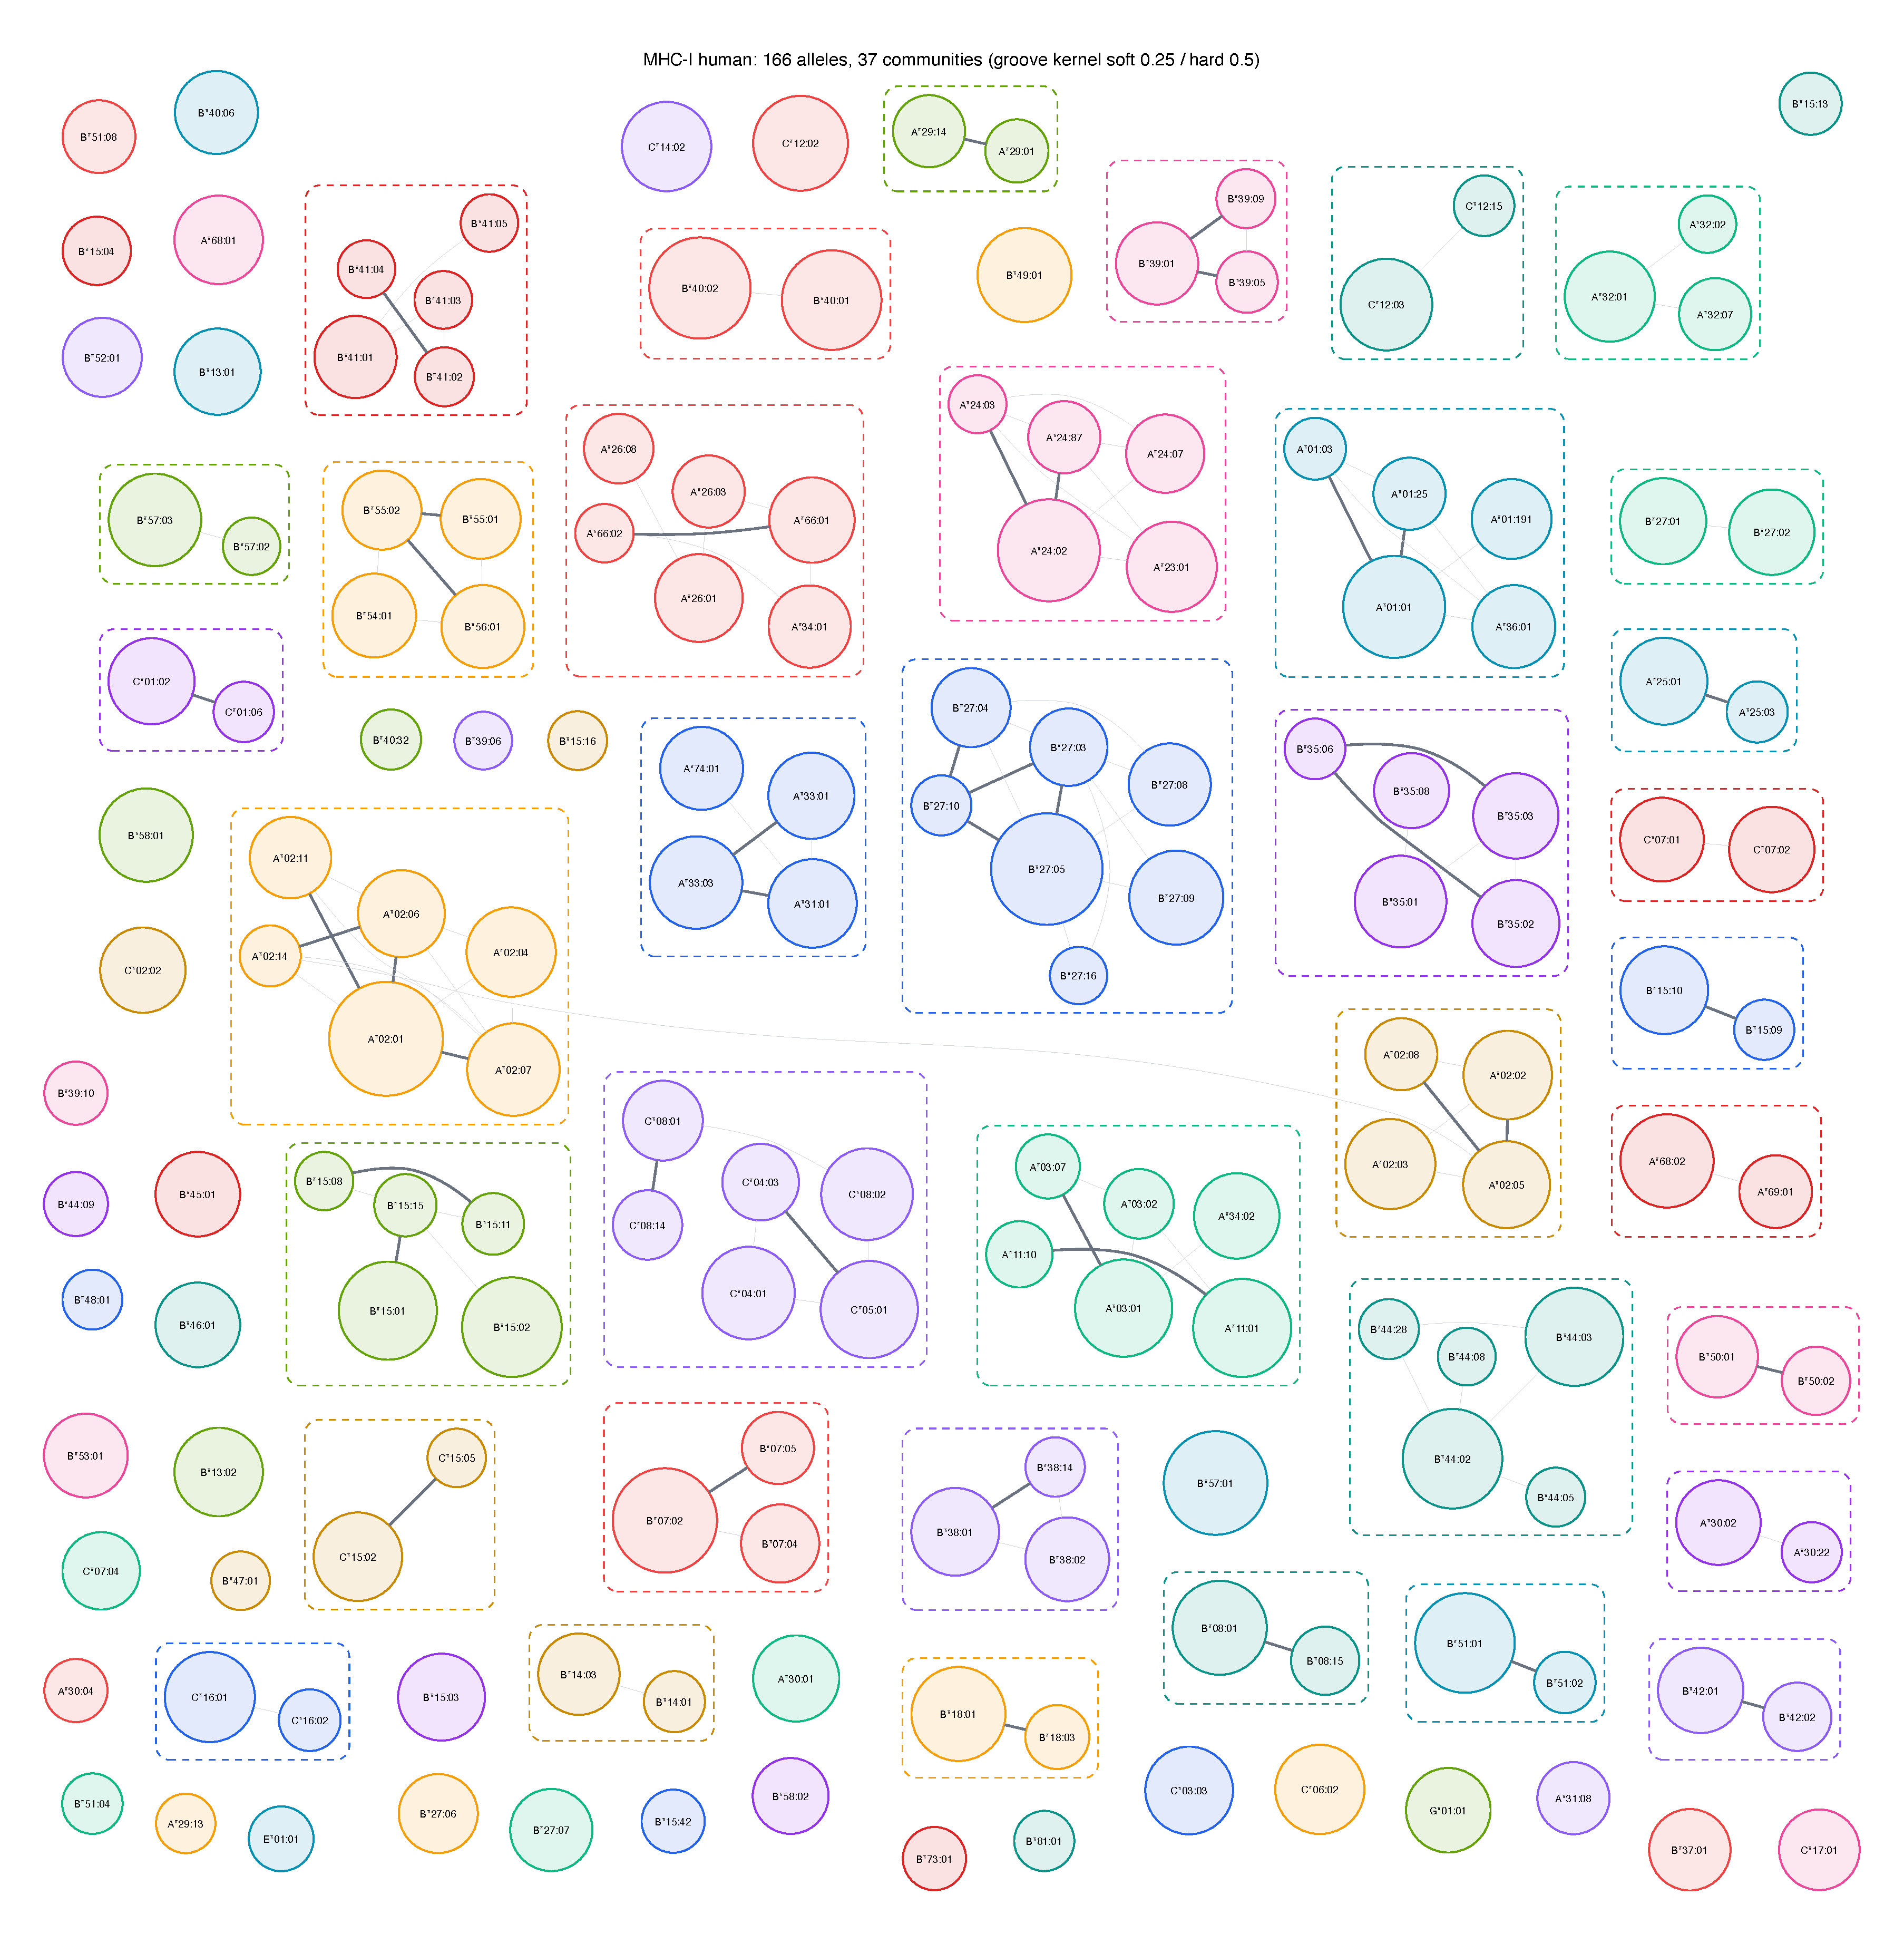
\includegraphics[width=0.92\linewidth]{promiscuity_mhc1_human.pdf}
  \caption{Human MHC-I allele network: nodes are alleles (size $\propto$ presented-set), edges the
  MI-weighted BLOSUM groove kernel~\eqref{eq:kernel} (thin $\ge0.25$, bold $\ge0.5$), dashed boxes
  the greedy-modularity communities. The communities recover known HLA-I supertypes. Mouse and
  class-II panels are generated likewise (\texttt{bench/promiscuity\_graph.py}).}
  \label{fig:promiscuity}
\end{figure}

An empirical counterpart (Figs.~\ref{fig:promiscuity-shared-human} and~\ref{fig:promiscuity-shared-mouse},
split by species) builds the same network from \emph{observed} co-presentation---edges are the overlap coefficient
$|P_a\cap P_b|/\min(|P_a|,|P_b|)$ of two alleles' presented-peptide sets---instead of predicted
groove similarity. Its communities agree with the supertypes, while the extra cross-community edges
are genuinely promiscuous peptides shared across distinct grooves; it covers alleles that lack a
pseudosequence (203 vs 166 human MHC-I) and even links the otherwise groove-divergent mouse alleles.
Quantifying predicted-vs-observed agreement, the Jaccard overlap of the two edge sets (over the
alleles common to both, human) is $0.19$ for MHC-I ($66/343$ edges) and $0.09$ for MHC-II
($42/458$): the groove kernel captures the high-confidence supertype core, while observed sharing is
broader and noisier. The two views are complementary rather than redundant.

\begin{figure}[ht]\centering
  \begin{subfigure}{0.49\linewidth}\includegraphics[width=\linewidth]{promiscuity_shared_mhc1_human.pdf}
    \caption{MHC-I}\end{subfigure}\hfill
  \begin{subfigure}{0.49\linewidth}\includegraphics[width=\linewidth]{promiscuity_shared_mhc2_human.pdf}
    \caption{MHC-II}\end{subfigure}
  \caption{\emph{Observed} \textbf{human} co-presentation networks (shared-epitope overlap
  coefficient; thin $\ge0.25$, bold $\ge0.5$; greedy-modularity communities). Communities are coarser
  than the predicted groove network (Fig.~\ref{fig:promiscuity}) because promiscuous peptides bridge
  supertypes. \texttt{bench/promiscuity\_graph.py}.}
  \label{fig:promiscuity-shared-human}
\end{figure}

\begin{figure}[ht]\centering
  \begin{subfigure}{0.49\linewidth}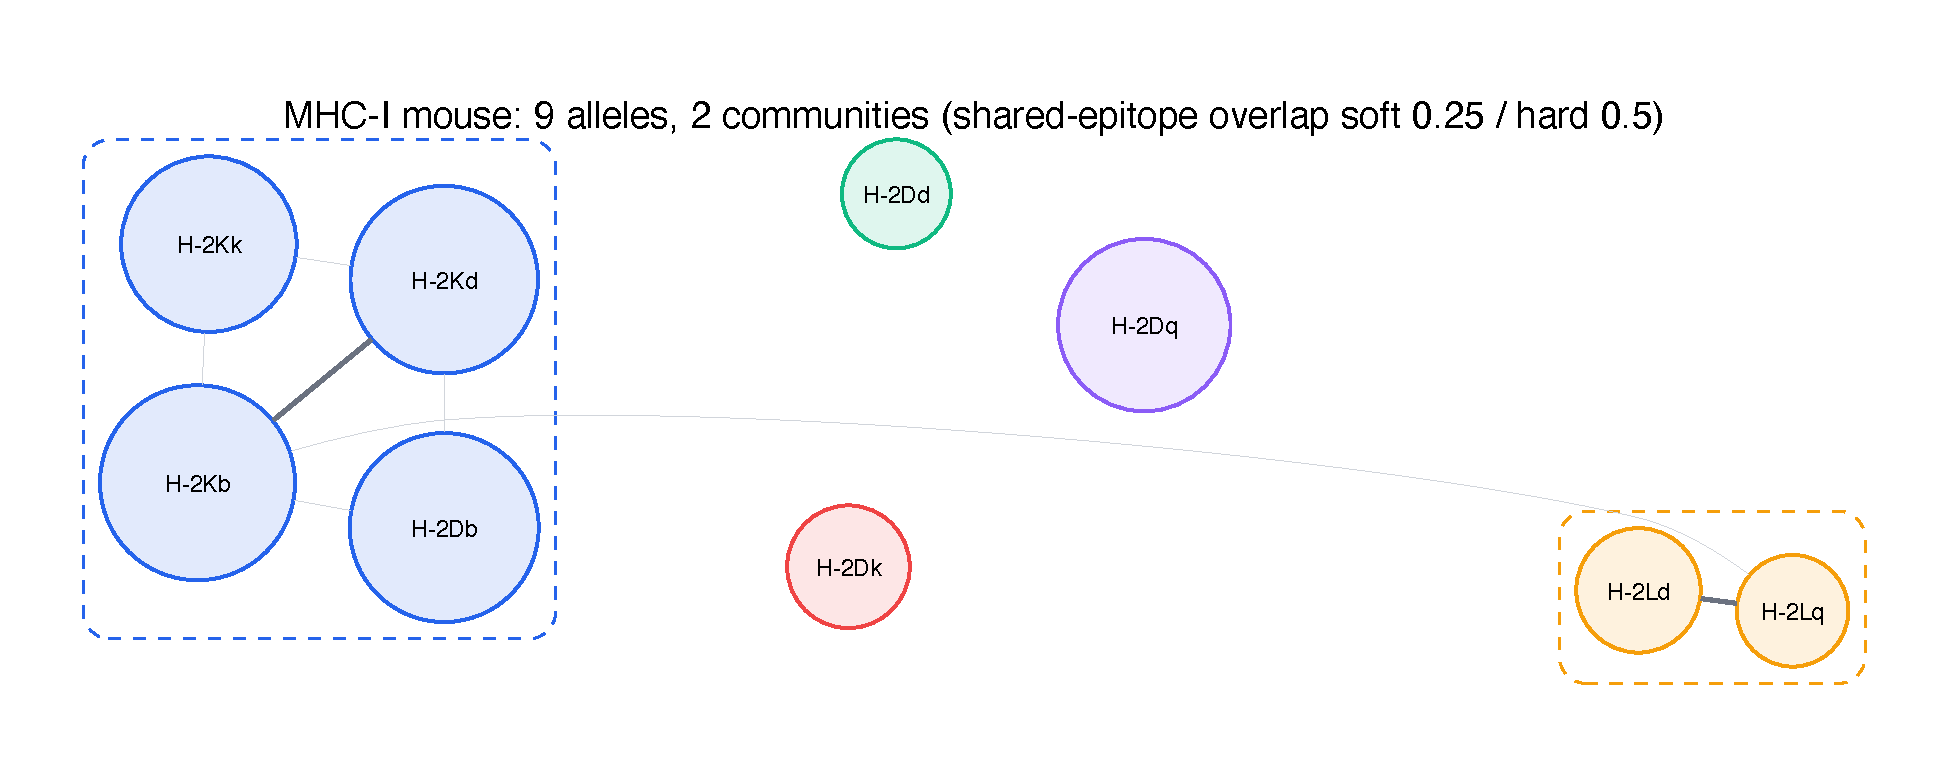
\includegraphics[width=\linewidth]{promiscuity_shared_mhc1_mouse.pdf}
    \caption{MHC-I}\end{subfigure}\hfill
  \begin{subfigure}{0.49\linewidth}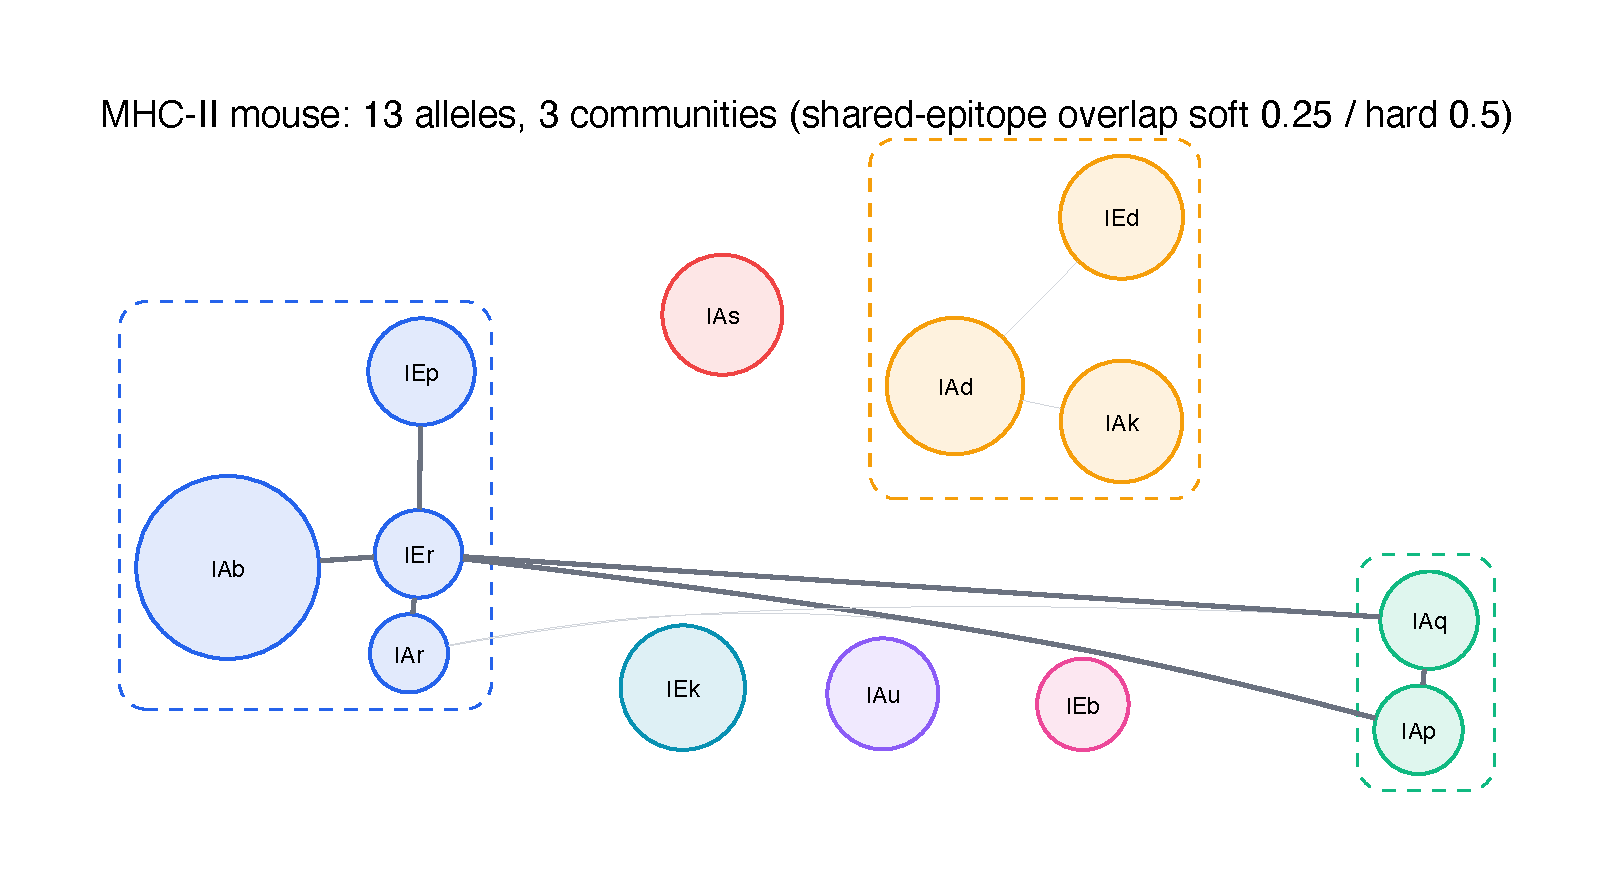
\includegraphics[width=\linewidth]{promiscuity_shared_mhc2_mouse.pdf}
    \caption{MHC-II}\end{subfigure}
  \caption{\emph{Observed} \textbf{mouse} co-presentation networks (shared-epitope overlap
  coefficient; same thresholds and method as Fig.~\ref{fig:promiscuity-shared-human}). Shared epitopes
  still link the groove-divergent mouse alleles, where the predicted groove kernel forms no
  communities. \texttt{bench/promiscuity\_graph.py}.}
  \label{fig:promiscuity-shared-mouse}
\end{figure}

\subsection{Per-pocket decomposition}\label{sec:pockets}
The anchor-factored weights~\eqref{eq:mi} make the pocket structure explicit: for each peptide anchor
we learn an independent weight vector $w_j$ over the 34 groove positions, per class and species
(Fig.~\ref{fig:pockets}, all four panels). Raw MI is inflated by \emph{linkage} between groove positions---they co-vary across alleles by
descent and structural co-evolution, so a position correlated with the true pocket residue also
scores high and the profile smears. We therefore prune indirect links by the data-processing
inequality (ARACNE~\cite{Margolin2006}): position $p$'s edge to pocket $j$ is dropped when another
position $q$ is more informative about both the pocket and $p$
($\MI(p;A_j)\le\min(\MI(q;A_j),\MI(p;q))$), leaving the \emph{direct} pocket positions. After
pruning, MHC-I (human) P$\Omega$/F-pocket collapses to a single dominant groove position ($\sim$19)
and P2/B-pocket to a small N-terminal cluster ($\sim$7--8), recovering the structural pocket layout
from presented-peptide statistics alone (Fig.~\ref{fig:pockets}). For MHC-II the relevance sits on
the polymorphic $\beta_1$ segment and is near-zero on the largely monomorphic $\alpha_1$ (sharpest for
DR, whose DRA $\alpha$ chain is invariant). The kernel itself keeps the \emph{un-pruned} MI weights
(the fuller signal gives marginally better neighbour matching---rare-allele recovery@5 $0.88$ vs
$0.85$ pruned); the prune is for interpretation. Mouse panels are data-limited ($8$--$13$ alleles),
noisier but with the same gross localization. (Class-II alleles are keyed by the $\alpha$--$\beta$
pair, cores from the register trick; its diffusion gain is small, $0.72\!\to\!0.74$ AUC.)

\paragraph{Structural validation.} The learned weights are confirmed by structure. We thread the
pseudosequence onto $372$ pMHC crystal structures (the \emph{Canonical2026} TCR:pMHC set) with a
fast C++ fitting aligner (\texttt{tcren.\_align}; no mmseqs/arda, $\sim$0.1\,s/structure) and count
peptide-anchor $\leftrightarrow$ groove-position heavy-atom contacts
(\texttt{bench/structural\_pockets.py}). Class is assigned per structure by which pseudosequence fits
best---an MHC-I 34-mer onto a single chain, or an MHC-II 34-mer onto the $\alpha_1$+$\beta_1$
chain-pair---rather than a $\beta_2$m/chain-length heuristic, which fails because TCR variable domains
($\sim$110\,aa) and class-II groove domains ($\sim$85\,aa) overlap $\beta_2$m's size and class-II
crystals are often domain-split; this yields $279$ MHC-I and $93$ MHC-II structures. For MHC-I the
contacts recover the learned layout from physics alone (Fig.~\ref{fig:structural})---P2 contacts
pseudosequence positions $\sim$7--8 (B-pocket), P$\Omega$ positions $\sim$15--17 (F-pocket),
overlapping the learned maxima---and
substituting these \emph{structural} contact-frequency weights into the kernel
(\texttt{weights="structural"}) gives near-identical rare-allele recovery@5 ($0.72$ vs $0.75$ learned,
5-fold CV): a data-independent prior agreeing with the data-learned one. For MHC-II the four core
pockets P1/P4/P6/P9 map to distinct $\alpha_1$+$\beta_1$ pseudosequence segments, and structural and
learned weights give indistinguishable (and near-neutral) recovery@5 ($0.464$ vs $0.465$)---confirming
that the small class-II diffusion gain is intrinsic to the harder class-II problem, not an artifact of
how the groove weights are estimated. A convex \emph{blend} (\texttt{weights="blend"}, structure as a
prior on the learned weights, $\tfrac12$ structural $+\tfrac12$ learned, renormalized) is the
principled empirical-Bayes choice when the learned weights are data-starved; on the current panels it
gives indistinguishable recovery@5 ($0.462$ vs $0.465$ learned for MHC-II, 5-fold CV), reinforcing the
same conclusion---more class-II ligand data, not a better weight estimator, is what the harder class
needs.

\begin{figure}[ht]\centering
  \begin{subfigure}{0.49\linewidth}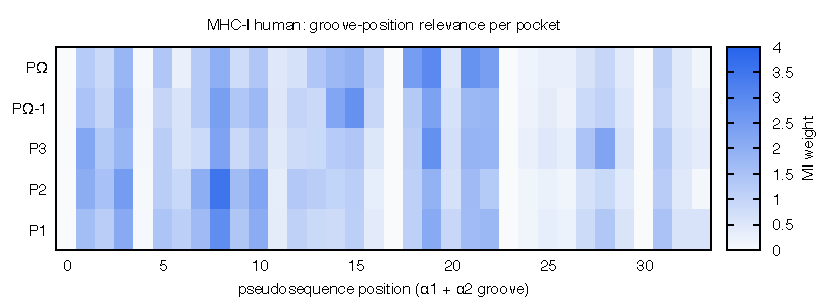
\includegraphics[width=\linewidth]{pockets_mhc1_human.pdf}
    \caption{MHC-I, human}\end{subfigure}\hfill
  \begin{subfigure}{0.49\linewidth}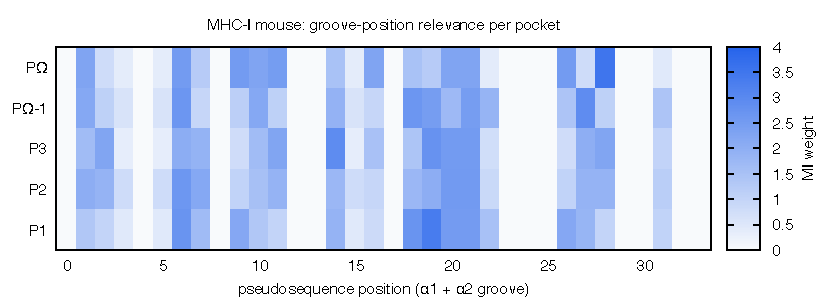
\includegraphics[width=\linewidth]{pockets_mhc1_mouse.pdf}
    \caption{MHC-I, mouse}\end{subfigure}

  \begin{subfigure}{0.49\linewidth}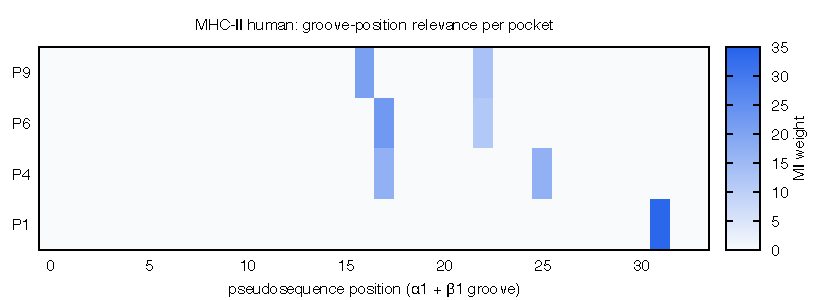
\includegraphics[width=\linewidth]{pockets_mhc2_human.pdf}
    \caption{MHC-II, human}\end{subfigure}\hfill
  \begin{subfigure}{0.49\linewidth}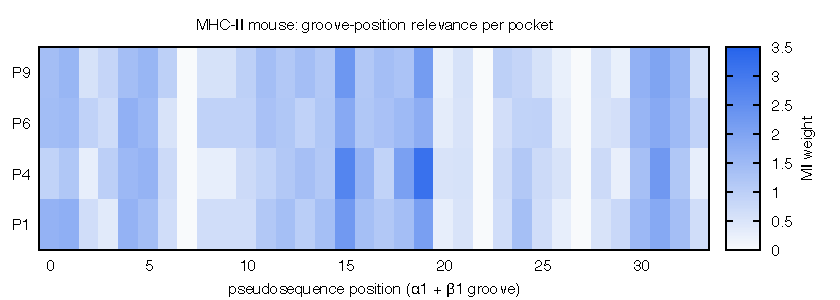
\includegraphics[width=\linewidth]{pockets_mhc2_mouse.pdf}
    \caption{MHC-II, mouse}\end{subfigure}
  \caption{Mutual-information relevance $w_{j,p}$ of each groove pseudosequence position $p$ (x) for
  each anchor pocket $j$ (rows), per class and species. Each panel shows raw MI (\emph{top}, blues)
  above the data-processing-inequality--pruned~\cite{Margolin2006} weights (\emph{bottom}, reds): raw
  MI is smeared by linkage between groove positions, while pruning keeps each pocket's \emph{direct}
  positions (MHC-I P$\Omega\to\sim$19, P2$\to\sim$7--8, disjoint); MHC-II concentrates on $\beta_1$.
  Colour scales are shared across all panels (one for raw, one for pruned) and winsorized at the
  $90$th percentile so the bulk of the scale stays legible. \texttt{bench/make\_figures.py}.}
  \label{fig:pockets}
\end{figure}

\begin{figure}[ht]\centering
  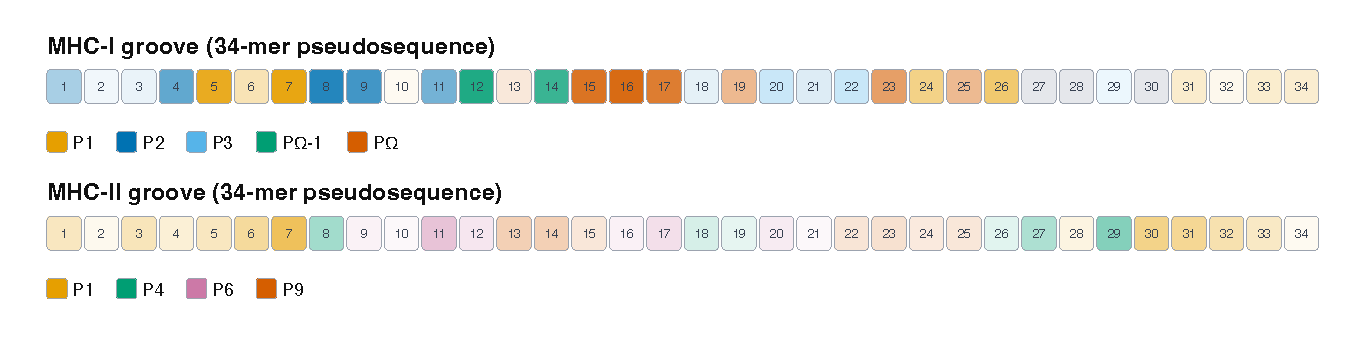
\includegraphics[width=0.96\linewidth]{structural_pockets.pdf}
  \caption{Structural pocket map: each of the $34$ groove pseudosequence positions coloured by the
  peptide anchor it contacts most across the pMHC crystals (\S\ref{sec:pockets}, $279$ MHC-I / $93$
  MHC-II structures), with opacity proportional to that heavy-atom contact frequency; pale grey marks
  positions with no appreciable peptide contact. The B-pocket (P2, $\sim$7--9) and F-pocket
  (P$\Omega$, $\sim$15--17) footprints emerge directly from structure and coincide with the pruned
  MI maxima of Fig.~\ref{fig:pockets}. Rendered in the residue-square style of \texttt{tcren}'s
  complementarity maps. \texttt{bench/structural\_figure.py}.}
  \label{fig:structural}
\end{figure}

\section{Proteome-scale matching}\label{sec:proteome}
\paragraph{Presentation scan.} To find all presented peptides in a protein we slide every
binding-length window (class~I $8$--$11$; class~II $\ge13$ with the register-anchored core) and
evaluate~\eqref{eq:conf} per window and allele. With $W$ windows and $|\mathcal A|$ panel alleles the
test is multiple: under the null the expected number of windows called for allele $a$ is
$\approx W\alpha$, so we control the family either by Bonferroni / max-statistic thresholds (FWER) or
by Benjamini--Hochberg on the $p_{\mathrm{enrich}}$ across the $W\times|\mathcal A|$ grid
(FDR)~\cite{Benjamini1995}. \texttt{scan\_protein(correction="bonferroni"|"bh")} applies exactly this
control over the voted $(window, allele)$ tests---Bonferroni for FWER, Benjamini--Hochberg for FDR---and
re-flags binders at the corrected threshold; ``correction=None`` keeps the per-window $\alpha$.

\paragraph{Same-MHC versus TCR-facing search.} At proteome scale two notions of ``similar peptide''
are distinguished by which mask of~\eqref{eq:masks} is indexed: \emph{same-MHC} similarity indexes
the presentation signature (peptides likely presented by the same allele), \emph{TCR-facing}
similarity indexes the anchor-masked central motif (similar T-cell recognition, the basis of
cross-reactivity). Both run on the C++ \texttt{KmerIndex} seed-and-gather.

\paragraph{Molecular mimicry.} A self or foreign peptide $p$ is a candidate cross-reactive mimic of a
neoantigen $\nu$ iff (i) it is presented by a compatible allele, (ii) the TCR-facing distance
$\dTCR(p,\nu)=\sum_i w_i\,\mathrm{pen}(p_i,\nu_i)\le\theta$ (anchors zeroed), and (iii) the hit is
significant against the per-allele presented background, $\widehat E\le\alpha$. Condition (iii)
deflates motifs common in the allele's peptidome and elevates surprisingly shared ones. This
connects to the neoantigen-quality program of \L{}uksza~et~al.: the quality $Q=R\times D$
\cite{Luksza2022,Luksza2017} multiplies a recognition / non-self term $R$ (the cross-reactivity
distance to known antigens) by a self-discrimination term $D$ (differential MHC binding), and to the
close-to-self ``shell'' picture of~\cite{TiffeauMayer2026}; \texttt{mhcmatch} supplies a calibrated
E-value for the $R$ component.

\paragraph{Near-exact source identification.} Given a neoantigen we identify the self peptide it
derives from---its parent protein and the mutated position---by full-sequence (unmasked)
$\le m$-mismatch search over all length-$L$ windows of the reference proteome. Under an
i.i.d.\ background of composition $\{q_c\}$ the expected number of chance windows within $m$
substitutions of a query in a proteome of $R$ residues is
\begin{equation}\label{eq:source}
  \E[\#\text{chance}]\approx R\sum_{i=0}^{m}\binom{L}{i}\bar q^{\,L-i}(1-\bar q)^{i},
  \qquad \bar q=\textstyle\sum_c q_c^2 ,
\end{equation}
the Karlin--Altschul/birthday count specialized to the Hamming ball (the empirical-background variant
reuses \texttt{seqtree} §KA). For $m\in\{0,1\}$ and $L\ge8$, \eqref{eq:source} is $\ll1$, so a hit is
essentially certainly the true source rather than coincidence---\texttt{Proteome.find\_source}
returns it with the differing residue flagged.

\section{Motif logos and length distributions}\label{sec:logos}
For an allele's presented set (class~I peptides of a fixed length; class~II register-anchored 9-mer
cores) the per-position information content is
\begin{equation}\label{eq:ic}
  I_i=\log_2 20-H_i-e(n_i),\qquad H_i=-\sum_{c}f_{i,c}\log_2 f_{i,c},
\end{equation}
with $f_{i,c}$ the residue frequency at position $i$ and $e(n_i)$ the small-sample entropy correction
for $n_i$ counts (negligible for the deep \texttt{pmhc\_data} alleles). The logo draws letter $c$ at
height $f_{i,c}I_i$ bits; columns at the anchors stand tall (e.g.\ A\*02:01 shows P2$=$L,
P$\Omega\in\{$V,L$\}$), the TCR-facing columns are flat. The length distribution is reported as a
companion histogram. Columns may be confidence-weighted by $n$ (or by the shortlist
$\ge2$-publication support). \texttt{logo.motif} returns the numeric logo; \texttt{logo.render} draws
it.

\section{Planned predictors and their composition}\label{sec:predictors}
Presentation is necessary but not sufficient for immunogenicity. Each planned predictor scores a
distinct biophysical or population term and \emph{composes} with the presentation evidence on the log
scale; for peptide $\sigma$ and allele $a$ the combined log-odds is
\begin{equation}\label{eq:combine}
  \log\frac{\Prob(\text{immunogenic})}{\Prob(\text{not})}
  = \beta_0
  + \beta_{\mathrm{pres}}\,(-\!\log p_{\mathrm{enrich}})
  + \beta_{\mathrm{aff}}\log\!\tfrac{1}{\mathrm{IC}_{50}}
  + \beta_{\mathrm{stab}}\,t_{1/2}
  + \beta_{\mathrm{clv}}\,c_{\mathrm{Cterm}}
  + \beta_{\mathrm{expr}}\log e_{\mathrm{gene}}
  + \beta_{\mathrm{imm}}\,\rho_{\mathrm{TCR}} ,
\end{equation}
with coefficients fit on labelled outcome data (the user will supply tuning/benchmark sets). The
terms: \emph{affinity} $\mathrm{IC}_{50}$ and \emph{stability} $t_{1/2}$ are the quantitative
complements of the binary presentation E-value, regressable on the same anchor features plus the
pseudosequence; \emph{cleavage} $c_{\mathrm{Cterm}}$ is a position-specific C-terminal generation
probability (with optional N-terminal trimming); \emph{expression} $e_{\mathrm{gene}}$ and variant
frequency enter as Bayesian priors multiplying the presentation odds; \emph{immunogenicity}
$\rho_{\mathrm{TCR}}$ combines physicochemical TCR-facing features with a TCR precursor-frequency
estimate in the $Q=R\times D$ spirit of~\cite{Luksza2022}. The precursor-frequency estimator is a
TCR-side quantity and is deferred to a separate package, consumed here only as a score. Each term is
a roadmap Phase-2 milestone specified by this subsection.

\section{Benchmark and evaluation methodology}\label{sec:bench}
We evaluate as a per-pMHC task: the unit is the (epitope, allele) pair. \emph{Exclusion is per-pMHC
and benchmark-only}---we hold out test (epitope, allele) pairs and drop \emph{only those pairs} from
training; the same epitope presented by a \emph{different} allele is a distinct, legitimate pMHC and
stays (so the model may borrow that co-presentation, exactly the cross-allele transfer the diffusion
is meant to exploit). We never exclude an epitope ``separately'' across alleles, and the production
model trains and votes on all data---the split exists only to score generalization. Matching counts
are \emph{punctured} for self-identity only (a query never counts itself, the $n^{>}$ convention of
the \texttt{seqtree} appendix). \emph{Metrics} are top-1 and top-5 accuracy and per-rarity \emph{recovery@5} (the
multi-label, promiscuity-aware score---top-1 is misleading when a peptide binds several alleles), the
per-(peptide,allele) ROC/PR-AUC, and a \emph{non-binder} baseline AUROC: the presentation score
(max over the panel) of real held-out peptides versus a matched set of $10{,}000$ random peptides
drawn at the corpus amino-acid frequency and length distribution. The latter establishes the floor
for non-binder rejection (real-vs-random AUROC $\approx0.80$ for human MHC-I, diffusion-neutral) and
is the negative class for the multi-class (allele $+$ non-binder) confusion matrix realized in
Fig.~\ref{fig:confusion} (\texttt{bench/confusion.py}). There each held-out peptide is assigned its
top-1 allele's \emph{locus} when the diffused score clears a gate calibrated to a $5\%$ non-binder
false-positive rate, else \emph{non-binder}. The model assigns the correct locus where it commits
(precision $0.62$--$0.65$ for HLA-A/B/C) and rejects $95\%$ of random peptides by construction, but a
single panel-max score gate cannot simultaneously reject non-binders and retain rare positives---top-1
recall falls to $0.17$--$0.32$ at $5\%$ FPR---because maximizing the per-allele log-odds over
$\sim$100 alleles inflates the family-wise false-positive rate. This is exactly why binder/non-binder
calling composes the per-allele score with the global $E_{\mathrm{glob}}$ gate (\S\ref{sec:evalue-role})
rather than thresholding one score. \emph{Comparison}: against NetMHCpan-4.1 and NetMHCIIpan-4.0
\cite{Reynisson2020}, MixMHCpred~\cite{BassaniSternberg2017}, and MixMHC2pred~\cite{Racle2019} on
matched alleles and shared eluted-ligand / assay test sets, with rank-threshold calibration and an
explicit \emph{rare-allele subgroup} analysis (the equity axis of~\cite{Glynn2025}) where the
pseudosequence diffusion is expected to help most. The benchmark datasets and the paper live in a
dedicated repository; this section fixes the protocol so it stays consistent with the predictors
defined here.

\begin{figure}[ht]\centering
  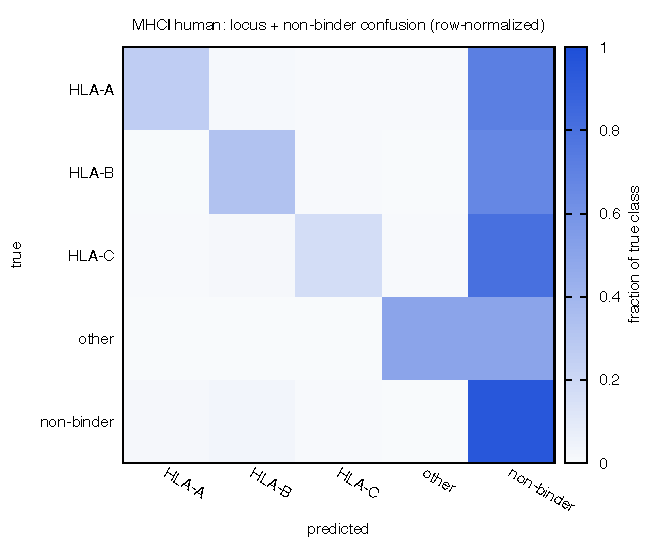
\includegraphics[width=0.6\linewidth]{confusion_mhc1_human.pdf}
  \caption{Human MHC-I locus $+$ non-binder confusion (row-normalized; \texttt{bench/confusion.py},
  shortlist tier). Each held-out peptide is assigned its top-1 allele's locus when the diffused score
  clears a gate calibrated to a $5\%$ non-binder false-positive rate, else \emph{non-binder}; the
  bottom row is $10{,}000$ corpus-AA random peptides (rejected at $95\%$ by construction). Locus
  assignment is accurate when the model commits (precision $0.62$--$0.65$), but the strict global gate
  costs top-1 positive recall---motivating the per-allele/global-$E$ composition of
  \S\ref{sec:evalue-role} over a single score threshold.}
  \label{fig:confusion}
\end{figure}

\paragraph{Performance.} Built on the C++ \texttt{KmerIndex}, the toolbox is fast enough for
proteome-scale use (\texttt{bench/bench\_speed.py}, one core, human MHC-I shortlist panel of $107$
alleles): a one-off store build of $1.4$\,s; allele restriction at $\sim$1900 peptides/s with
diffusion (rank all alleles) and $\sim$4000/s by vote; a $596$-aa protein scan in $0.3$\,s;
TCR-facing similarity search of $2\times10^4$ peptides in $40$\,ms; and proteome source lookup in
$\sim$60\,ms, at $\sim$0.6\,GB peak.

\section{Assumptions and limitations}\label{sec:limits}
(i) The analytic pooled null assumes approximate position independence in the anchor block; real
co-occupancy adds a two-point ($b_2$) correction (the negative-binomial tail of the \texttt{seqtree}
appendix) that keeps the mean robust while inflating the tail. (ii) Kernel validity rests on a
faithful pseudosequence; ambiguous (\texttt{X}) positions are skipped and locus-aware normalization
of allele names is required (class~II especially). (iii) The pooled E-value is a smoothed estimator
(Prop.~\ref{prop:bv})---its bias must be reported alongside the gain for rare alleles. (iv) The
class-II register trick is a one-pass proxy for full deconvolution~\cite{Andreatta2017,Alvarez2019}.
(v) ``Compatible allele'' in mimicry is a user input; cross-reactivity significance is conditional on
a faithful per-allele presented control. These are the open items tracked in \texttt{ROADMAP.md}.

\bibliographystyle{plain}
\bibliography{refs}

\end{document}
